\paragraph{GET /:lang/user/training/question} % richiesta che ritorna la prossima domanda dell'allenamento
\begin{itemize}
\item \textbf{Successo}
% descrizione diagramma e UML

\textbf{Descrizione}: il \texttt{QuestionRouter} gestisce la richiesta \textit{REST\ped{G}} del Front-End passando il controllo al \texttt{TopicController}; viene poi invocato il metodo\\ \texttt{getNextQuestion(req,res,next)} che ritorna la prossima domanda da sottoporre all'utente durante l'Allenamento. 

\begin{figure}[ht]
	\centering
	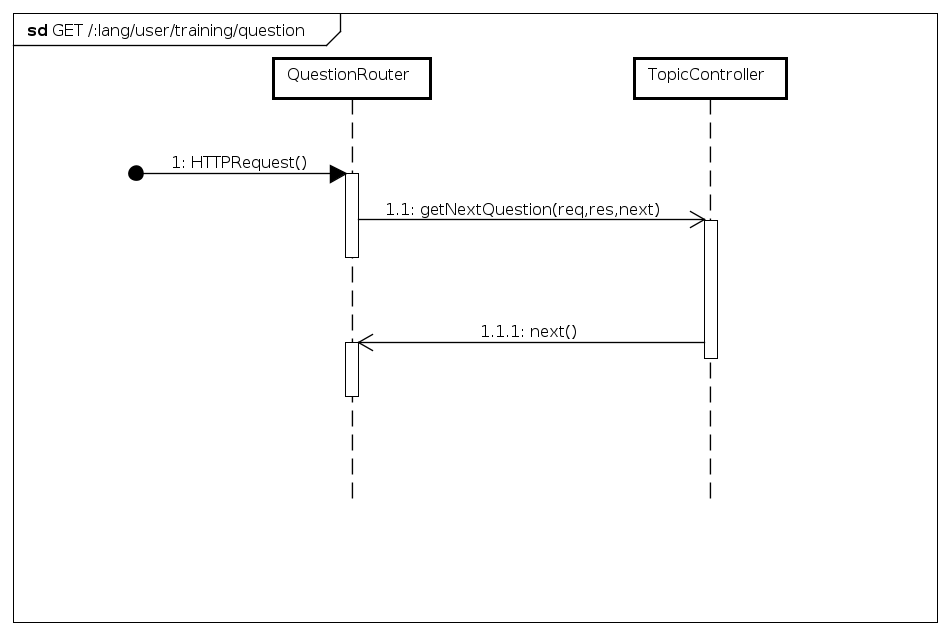
\includegraphics[scale=0.45]{UML/DiagrammiDiSequenza/Back-end/GET__lang_user_training_question.png}
	\caption{GET /:lang/user/training/question}
\end{figure}
\FloatBarrier

\item \textbf{Fallimento}
% descrizione diagramma e UML
\end{itemize}




\paragraph{PUT /:lang/user/training/userstatistics} % richiesta che aggiorna le statistiche dell'utente
\begin{itemize}
\item \textbf{Successo}
% descrizione diagramma e UML

\textbf{Descrizione}: lo \texttt{UserRouter} gestisce la richiesta \textit{REST\ped{G}} del Front-End passando il controllo allo \texttt{UserManagementController}; viene poi invocato il metodo\\ \texttt{UpdateStatisticsUser(req,res,next)} che aggiorna le statistiche dell'utente che ha risposto alla domanda.

\begin{figure}[ht]
	\centering
	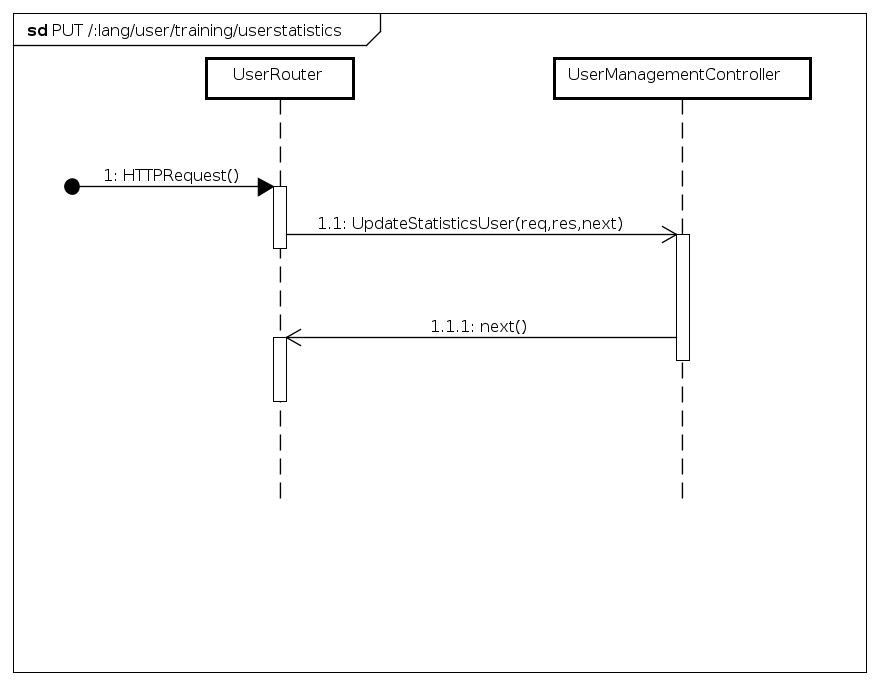
\includegraphics[scale=0.45]{UML/DiagrammiDiSequenza/Back-end/PUT__lang_user_training_userstatistics.png}
	\caption{PUT /:lang/user/training/userstatistics}
\end{figure}
\FloatBarrier

\item \textbf{Fallimento}
% descrizione diagramma e UML
\end{itemize}




\paragraph{PUT /:lang/user/training/questionstatistics} % richiesta che aggiorna le statistiche della domanda
\begin{itemize}
\item \textbf{Successo}
% descrizione diagramma e UML

\textbf{Descrizione}: il \texttt{QuestionRouter} gestisce la richiesta \textit{REST\ped{G}} del Front-End passando il controllo al \texttt{QuestionController}; viene poi invocato il metodo\\ \texttt{updateStatistics(req,res,next)} che aggiorna le statistiche della domanda a cui è appena stata data una risposta.

\begin{figure}[ht]
	\centering
	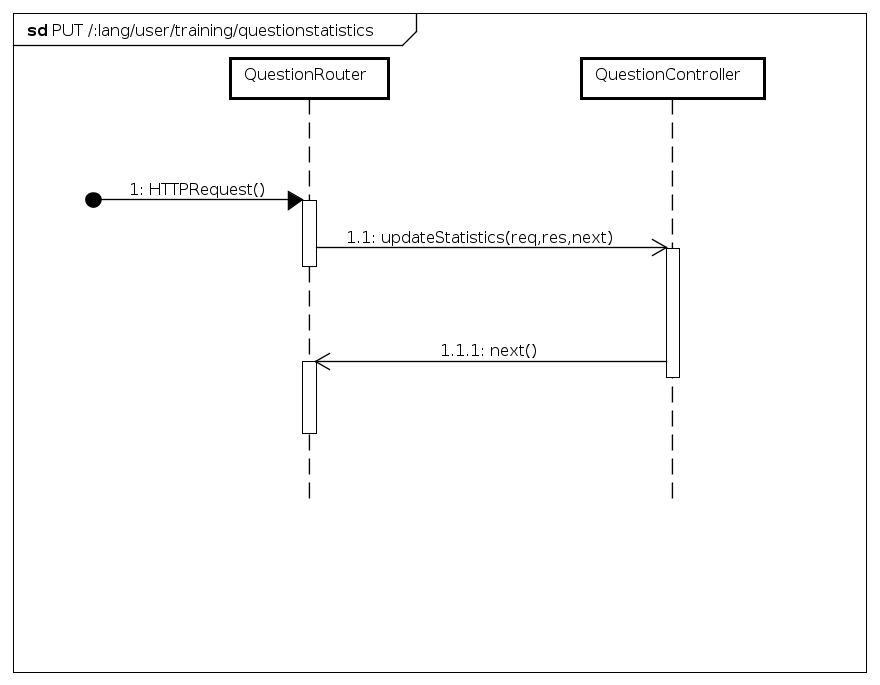
\includegraphics[scale=0.45]{UML/DiagrammiDiSequenza/Back-end/PUT__lang_user_training_questionstatistics.png}
	\caption{PUT /:lang/user/training/questionstatistics}
\end{figure}
\FloatBarrier

\item \textbf{Fallimento}
% descrizione diagramma e UML
\end{itemize}  